\section{Évaluation de l'hypothèse de pertinence}
\label{section:4.4-HYPOTHESE-PERTINENCE}

	%%% Introduction / Transition.
	Jusqu'à présent, nous avons analysé la performance et l'évolution des résultats de notre implémentation du \textit{clustering} interactif à l'aide d'une vérité terrain (cf. calcul de \texttt{v-measure}).
	Cependant, une telle référence n'est pas accessible en situation réelle (l'objectif de notre méthode est précisément de la construire).
	Nous devons donc nous intéresser à d'autres moyens d'estimer la pertinence des bases d'apprentissages obtenus et de définir comment définir l'exploitabilité d'un résultat.
	Ainsi, nous aimerions vérifier l'hypothèse suivante :
	
	%%% Formulation des hypothèses:
	\begin{tcolorbox}[
		title=\faVial~\textbf{Hypothèse de pertinence}~\faVial,
		colback=colorTcolorboxHypothesis!15,
		colframe=colorTcolorboxHypothesis!75,
		width=\linewidth
	]
		« \textbf{
			Au cours d'une méthodologie d'annotation basée sur le \textit{clustering} interactif, il est possible à un expert métier d'évaluer rapidement la pertinence de la base d'apprentissage en construction sans utiliser de vérité terrain.
		} » \\
		
		% Figure.
		La figure~\ref{figure:4.4-HYPOTHESE-PERTINENCE} illustre cette hypothèse et l'espoir de pouvoir caractériser la qualité de la base d'apprentissage en cours de construction en fonction d'une valeur métier exprimée par un expert.
		%
		\begin{figure}[H]  % keep [H] to be in the tcolorbox.
			\centering
			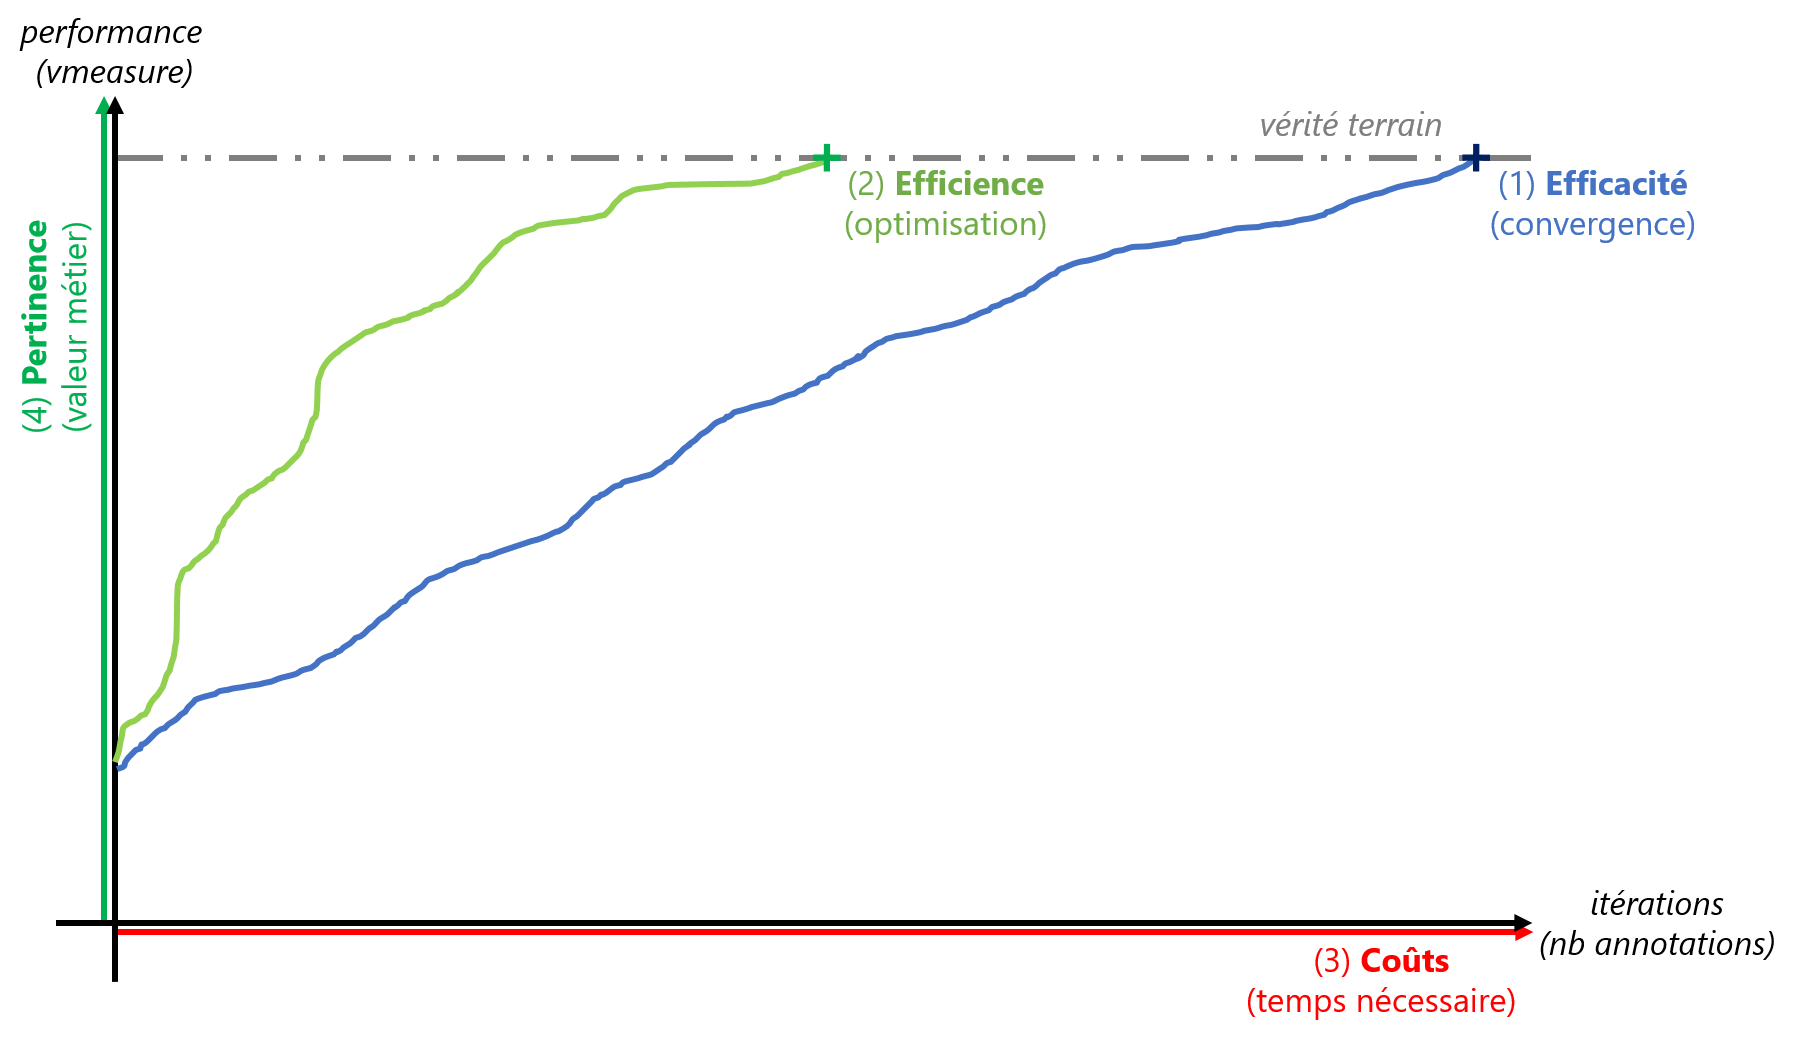
\includegraphics[width=0.95\textwidth]{figures/hypotheses-04-pertinence}
			\caption{Illustration des études réalisées sur le \textit{clustering} interactif (\textit{étape 4/6}) en schématisant l'évolution de la pertinence (\textit{valeur métier évaluée par l'expert et exprimé en nombre de clusters}) d'une base d'apprentissage en cours de construction en fonction du coût temporel de la méthode (\textit{temps nécessaire à l'expert métier et à la machine}).}
			\label{figure:4.4-HYPOTHESE-PERTINENCE}
		\end{figure}

	\end{tcolorbox}
		
	% Résumé de l'étude.
	Afin de vérifier cette hypothèse, nous explorons trois approches :
	\begin{itemize}
		\item une \textbf{vérification par un expert} du partitionnement des données obtenus, en parcourant manuellement le contenu des \textit{clusters} et en donnant un avis sur l'exploitabilité de ces derniers (cf. sous-section~\ref{section:4.4.1-ETUDE-PERTINENCE-VERIFICATION-MANUELLE}) ;
		\item une analyse des \textbf{patterns linguistiques saillants} dans la base d'apprentissage à l'aide d'une stratégie de sélection des composantes principales d'un modèle (cf. sous-section~\ref{section:4.4.2-ETUDE-PERTINENCE-PATTERNS-LINGUISTIQUES}),
		\item et une approche utilisant un \textbf{résumé automatique de thématique} par un modèle de langue, permettant de décrire succinctement le contenu des \textit{clusters} en une phrase. (cf. sous-section~\ref{section:4.4.3-ETUDE-PERTINENCE-RESUME-AUTOMATIQUE}).
	\end{itemize}
	
	
	%%%
	%%% Subsection 4.4.1: Étude d'une vérification manuelle de la valeur métier d'une base d'apprentissage par un expert
	%%%
	\subsection{Étude d'une vérification manuelle et non assistée de la valeur métier d'une base d'apprentissage par un expert}
	\label{section:4.4.1-ETUDE-PERTINENCE-VERIFICATION-MANUELLE}
		
		% Objectif de l'expérience.
		Afin d'estimer la pertinence d'un résultat de \textit{clustering}, notre première intuition consiste à demander simplement l'avis d'un expert sur la base d'apprentissage en cours de construction.
		En lui posant certaines questions, nous espérons obtenir une description qualitative de chaque \textit{cluster} et ainsi déduire quand le résultat du \textit{clustering} interactif devient exploitable pour définir et entraîner un modèle de classification.
	
		%%% Protocole expérimental.
		\subsubsection{Protocole expérimental}
			
			% Pseudo-code.
			Pour résumer le protocole expérimental que nous décrivons ci-dessous, vous pouvez vous référer au pseudo-code décrit dans Alg.~\ref{algorithm:4.4.1-ETUDE-PERTINENCE-VERIFICATION-MANUELLE-PROTOCOLE}.
			%
			\begin{algorithm}[!htb]
				\begin{algorithmic}[1]
					\Require jeux de données annotés (vérité terrain) de tailles différentes
					\State \textbf{initialisation (données)}: récupérer ou générer les données et la vérité terrain
					\State \textbf{initialisation (contraintes)}: créer une liste vide de contraintes
					\State \textbf{prétraitement}: supprimer le bruit dans les données avec \texttt{prep.simple}
					\State \textbf{vectorisation}: transformer les données en vecteurs avec \texttt{vect.tfidf}
					\State \textbf{clustering initial}: regrouper les données par similarité avec \texttt{clust.kmeans.cop}
					\State \textbf{évaluation manuelle}: juger de l'exploitabilité de chaque \textit{cluster}
					\Repeat
						\State \textbf{échantillonnage}: sélectionner de nouvelles contraintes à annoter
						\State \textbf{simulation d'annotation}: ajouter des contraintes avec \texttt{samp.closest.diff}
						\State \textbf{clustering}: regrouper les données par similarité avec \texttt{clust.kmeans.cop}
						\State \textbf{évaluation manuelle}: juger de l'exploitabilité de chaque \textit{cluster}
						\State \textbf{labellisation manuelle}: nommer chaque \textit{cluster} exploitable
					\Until{annotation de toutes les contraintes possibles}
					\State \textbf{analyse}: afficher l'évolution de l'exploitabilité de chaque itération de \textit{clustering}
					\Ensure discussion sur la complexité de la tâche et sur l'évolution de l'exploitabilité
				\end{algorithmic}
				\caption{Description en pseudo-code du protocole expérimental de l'étude de vérification manuelle non assistée de la valeur métier d'une base d'apprentissage.}
				\label{algorithm:4.4.1-ETUDE-PERTINENCE-VERIFICATION-MANUELLE-PROTOCOLE}
			\end{algorithm}
			
			% Description de la vérité terrain.
			Nous utilisons comme vérité terrain le jeu de données \texttt{Bank Cards (v1.0.0)} : ce dernier traite des demandes les plus fréquentes des clients en ce qui concerne la gestion de leur carte bancaire.
			Il est composé de $500$ questions rédigées en français et réparties en $10$ classes (\texttt{perte ou vol de carte}, \texttt{carte avalée}, \texttt{commande de carte}, ...).
			Pour plus de détails, consultez l'annexe~\ref{annex:C.1-DATASET-BANK-CARDS}.
			
			% Description des tentatives de la méthode.
			Sur ce jeu de données, nous exécutons une tentative complète
			\footnote{Tentative complète : itérations d'échantillonnage, d'annotation et de \textit{clustering} jusqu'à annotation de toutes les contraintes possibles.}
			de la méthode du \textit{clustering} interactif utilisant notre paramétrage favori, et cette tentative est répétée $5$ fois pour contrer les aléas statistiques des exécutions.
			
			% Description de l'évaluation manuelle.
			Au cours des itérations, un expert qualifie chaque \textit{cluster} en donnant son avis sur sa valeur métier.
			Afin d'encadrer ses réponses, nous lui demandons d'analyser trois aspects :
			\begin{itemize}
				\item est-ce que le \textit{cluster} a une thématique principale \textbf{bien définie} ? (\textit{en effet, comment interpréter un cluster sans définition claire ?})
				\item est-ce que le \textit{cluster} est constitué par un nombre suffisant de données ? (\textit{en effet, comment entraîner un modèle de classification sans données ?})
				\item est-ce que le \textit{cluster} n'est pas trop bruité ? (\textit{en effet, comment avoir de bonnes performances si la base d'apprentissage n'est pas fiable ?})
			\end{itemize}
			
			L'avis exprimé par l'expert métier est alors classé en trois niveaux :
			\begin{itemize}
				\item \textbf{exploitable} : le \textit{cluster} possède (1) une thématique bien définie, (2) un nombre de données suffisant pour entraîner un modèle de classification et (3) peu de bruit ; ce \textit{cluster} peut donc être exploité en l'état ou avec peu de modifications manuelles ;
				\item \textbf{partiellement exploitable} : soit le \textit{cluster} est composé de plusieurs de thématiques (\textit{deux ou trois}), soit il ne comporte pas pas assez de données (\textit{moins d'une vingtaines}), soit il est bruité (\textit{au moins un quart de bruit}) ; ce \textit{cluster} donne une première base pour créer une classe, mais un travail manuel est nécessaire (\textit{ajout de données, tri du bruit, ...}) ;
				\item \textbf{non exploitable} : soit le \textit{cluster} ne contient pas ou contient trop de thématique, soit c'est un \textit{cluster} singleton ou un \textit{cluster} poubelle, soit ce \textit{cluster} est complètement bruité ; dans tous les cas, il n'est absolument pas exploitable sans un gros travail manuel.
			\end{itemize}
			
			Pour limiter la charge de travail de l'opérateur, nous ne demandons l'expertise que toutes les $5$ itérations d'une tentative.
			
			% Référence scripts.
			\begin{leftBarInformation}
				Les scripts de l'expérience, réalisés avec des \textit{notebooks} Python (\cite{van-rossum-drake:2009:python-reference-manual}), sont disponibles dans un dossier dédié de~\cite{schild:2021:cognitivefactory-interactiveclusteringcomparativestudy}.
			\end{leftBarInformation}
			

		%%% Résultats
		\subsubsection{Résultats obtenus}
			
			% Axiome/Contraintes.
			\begin{leftBarWarning}
				Par manque de personnes aptes à qualifier le jeu de données utilisé, les annotations réalisées dans cette étude n'ont pu être faites que par un seul annotateur.
				Malgré cette contrainte, nous supposons que la réalisation de l'analyse sur $5$ tentatives différentes de la méthode permet de limiter les biais et de discuter des tendances générales.
			\end{leftBarWarning}
		
			% Description statistiques.
			La figure~\ref{figure:4.4.1-ETUDE-PERTINENCE-VERIFICATION-MANUELLE} met en avant l'évolution de le pertinence moyenne estimée par l'opérateur sur la base des contenu des \textit{clusters}.
			Nous allons nous intéresser à trois phases s'y distinguant.
			
			% 0: Initialisation
			À l'initialisation (itération $0$), la majeure partie des \textit{clusters} sont inexploitables (environ $60$\%) et seul $35$\% d'entre eux semblent exploitables.
			Dans le top $3$ des classes facilement identifiables à ce stade, nous retrouvons \texttt{gestion\_sans\_contact} ($5/5$), \texttt{consultation\_solde} ($3/5$) et \texttt{gestion\_carte\_virtuelle} ($3/5$).
			
			% 0-10: Phase d'exploration.
			Nous constatons ensuite une première phase de remaniement des \textit{clusters}, située entre les itérations $0$ et $10$, où le taux d'inexploitables chute au profit des \textit{clusters} partiellement exploitables, dont la proportion augmente de $10$ à près de $40$\%.
			À l'itération $10$, le top $3$ des classes identifiables mais bruitées ou en cohabitation dans un \textit{cluster} sont \texttt{gestion\_carte\_virtuelle} ($4/5$),  \texttt{alerte\_perte\_vol\_carte} ($4/5$) et  \texttt{commande\_carte} ($4/5$).
			
			% 10-25: Phase de consolidation.
			Une seconde phase de consolidation se présente entre les itérations $10$ et $25$.
			Durant cette phase, les taux de \textit{clusters} non exploitables et de partiellement exploitables diminuent alors que le taux d'exploitables monte en flèche (de $35$\% à $90$\% en $15$ itérations).
			La majeure partie des \texttt{clusters} sont ainsi exploitables en l'état ou après la correction de quelques points aberrants.
			Après l'itération $25$, le \textit{cluster} le plus récalcitrant concerne un mélange des classes \texttt{alerte\_perte\_vol\_carte} et \texttt{gestion\_decouvert} ($5/5$).

			% Figure.
			\begin{figure}[!htb]
				\centering
				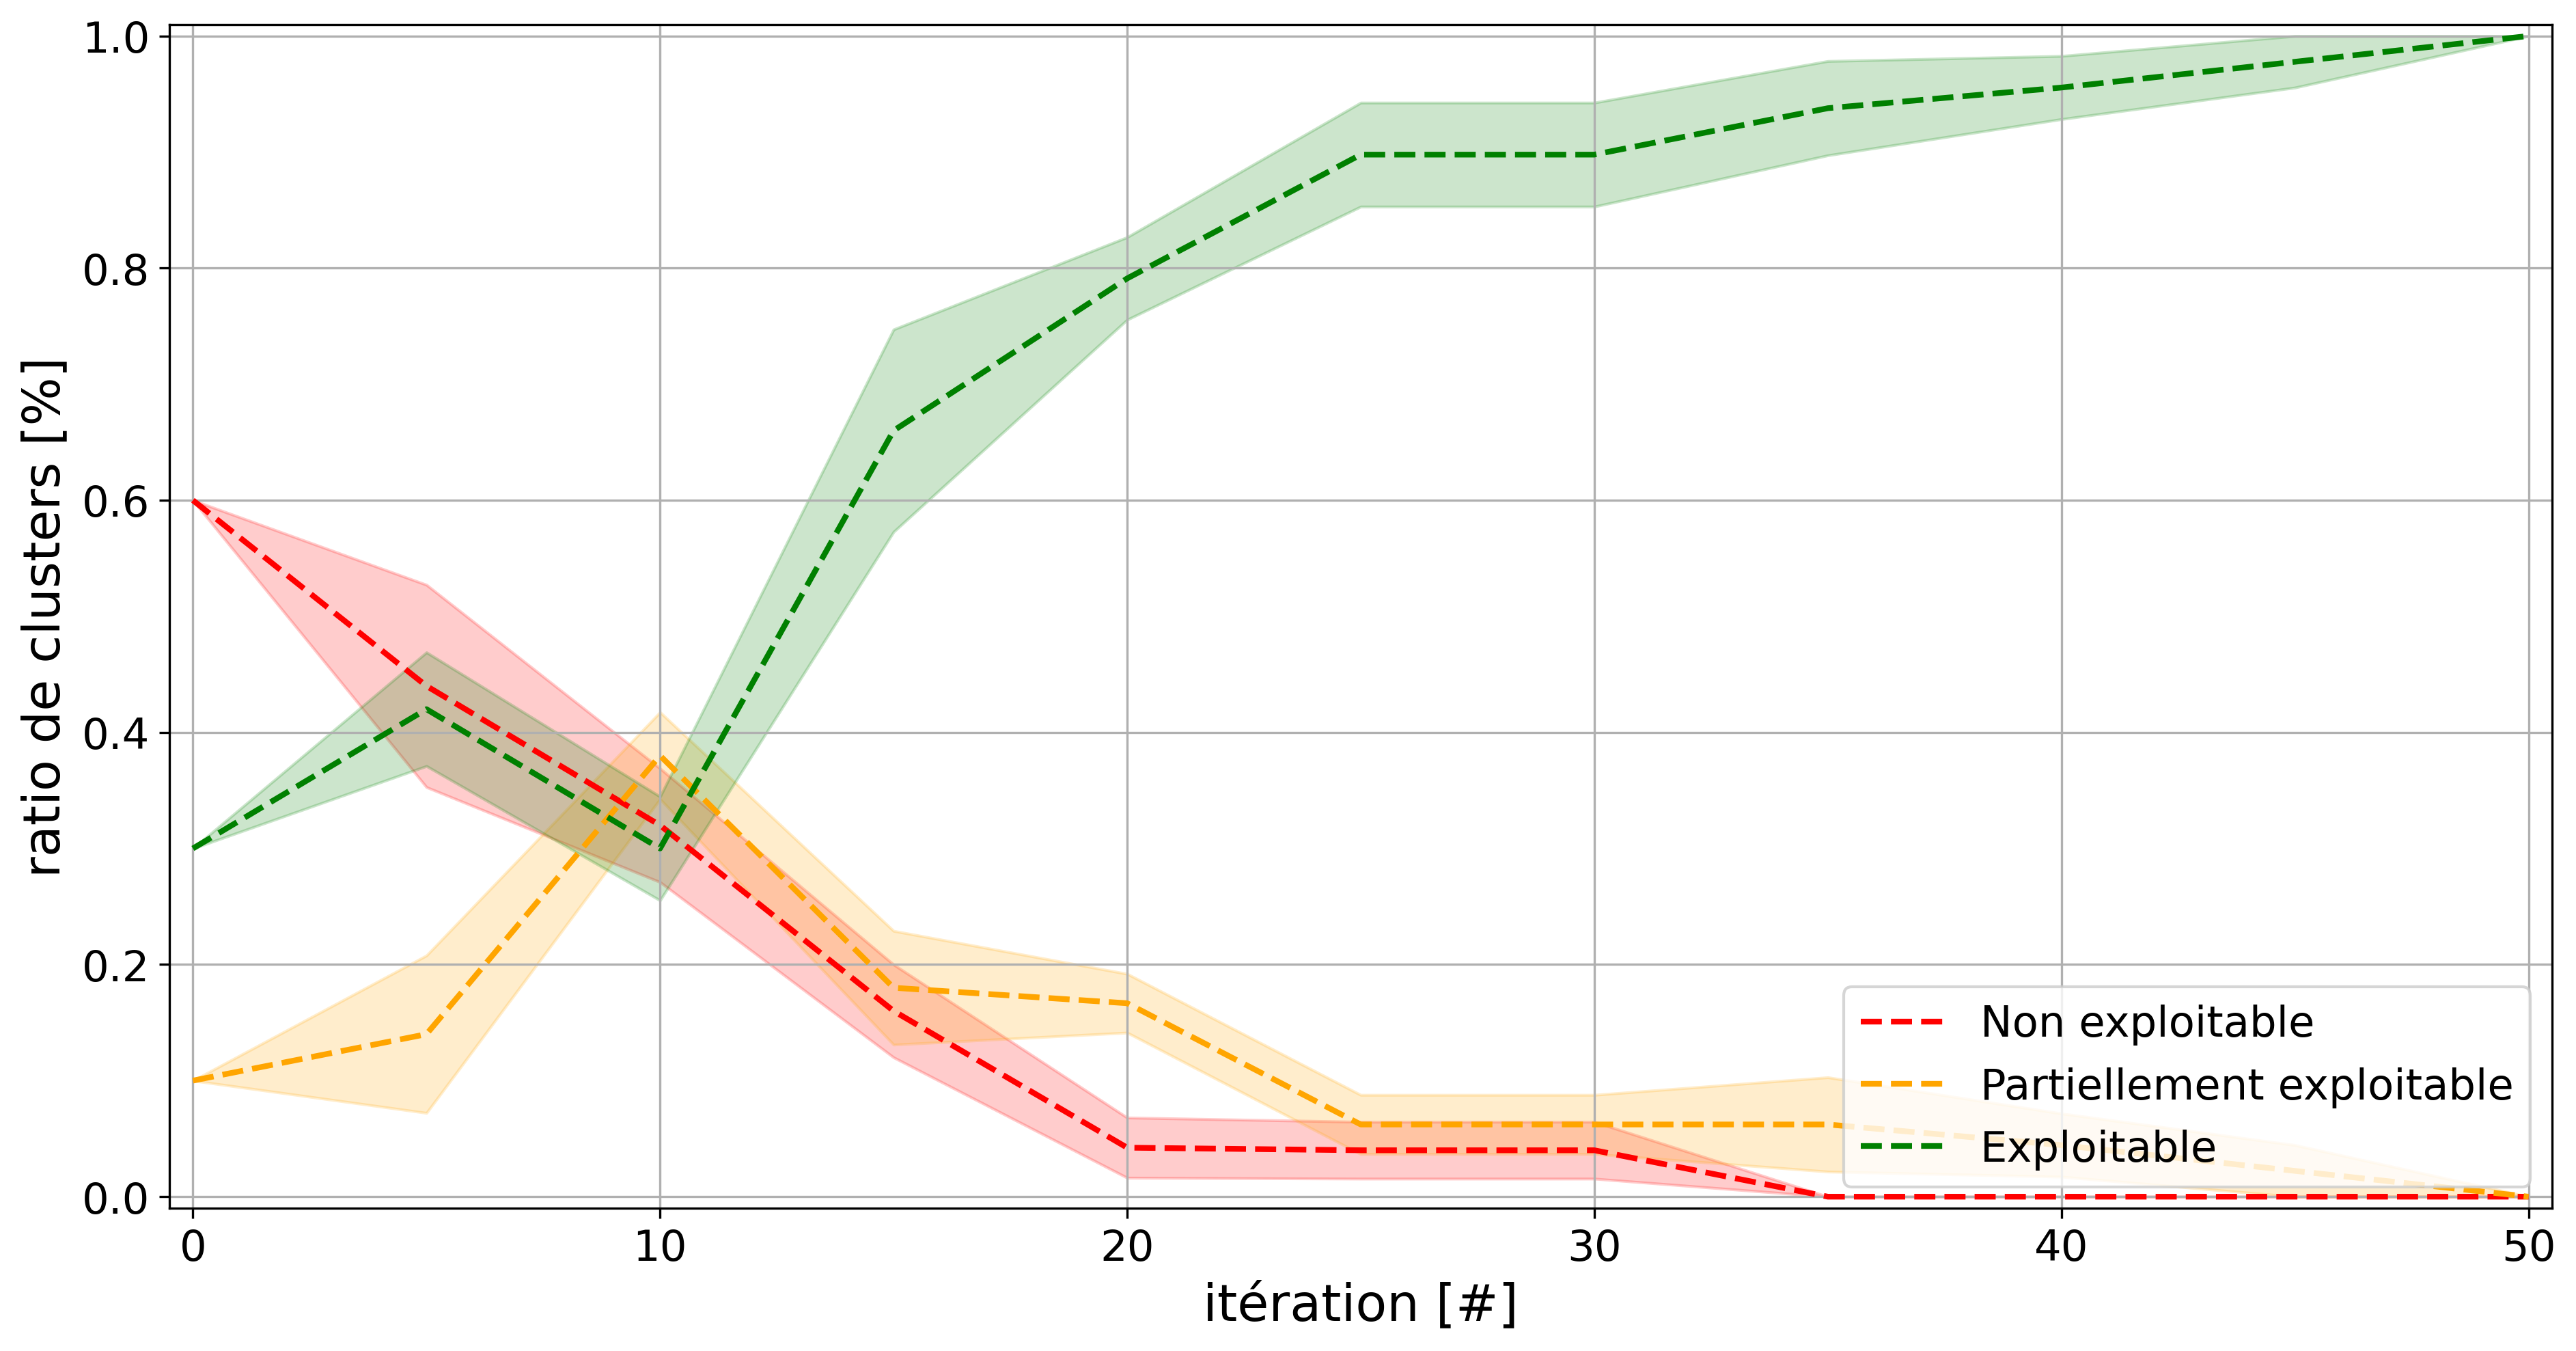
\includegraphics[width=0.95\textwidth]{figures/etude-pertinence-llm-check-clustering-annotation-favori}
				\caption{Évolution de la pertinence métier moyenne estimée manuellement au cours des itérations du résultat du \textit{clustering} interactif avec notre paramétrage favori.
				Cette pertinence, exprimée en proportion du nombre de \textit{clusters}, est retranscrite en trois niveaux : \texttt{exploitable} en vert, \texttt{partiellement exploitable} en orange, et \texttt{non exploitable} en rouge.}
				\label{figure:4.4.1-ETUDE-PERTINENCE-VERIFICATION-MANUELLE}
			\end{figure}


		%%% Discussion
		\subsubsection{Discussion}
		
			% Rappel de l'objectif.
			Cette première étude visait à observer comment un expert métier peut interpréter un résultat de \textit{clustering} proposé par notre méthode.
			
			% Remarques sur l'évolution de l'exploitabilité.
			Comme l'analyse n'a pu être faite que par un seul opérateur, nous ne nous attarderons pas sur la précision des taux d'exploitabilité des clusters.
			Nous pouvons déjà reconnaître que trois phases sont présentes :
			\begin{itemize}
				\item une première \textbf{phase exploratoire} (cf. itérations $0$ à $10$), où de premiers \textit{clusters} partiellement exploitables apparaissant.
				Ces derniers contiennent souvent une thématique bruitée ou quelques thématiques mal séparées, ce qui permet toutefois à l'expert de se faire une idée des thématiques contenu dans la collecte de données.
				Cependant, s'arrêter à ce stade demanderait beaucoup de travail manuel pour obtenir une base d'apprentissage opérationnelle ;
				\item une seconde \textbf{phase de consolidation} (cf. itérations $10$ à $25$), où les \textit{clusters} partiellement exploitable se raffinent.
				De plus en plus de \textit{clusters} bien définis naissent, avec une seul thématique et peu de bruits.
				Ces derniers pourraient être extraits et exploités en l'état ;
				\item une \textbf{phase de parachèvement} (cf. itérations après $25$), où la plupart des \textit{clusters} sont exploitables en l'état mais quelques-uns nécessitent encore du travail.
				Cette phase est la moins rentable car les derniers \textit{clusters} et points aberrants sont corrigés petit à petit, mais sans impact notable sur leur valeur métier. 
			\end{itemize}
			
			% Remaques expérience utilisateur : tâche complexe.
			Au cours de ces vérifications, il apparaît que la complexité réside dans l'analyse des \textit{clusters} partiellement exploitables.
			En effet, les clusters totalement exploitable ou totalement inexploitables sont souvent simples à identifier.
			les premiers se repèrent facilement, surtout quand ils sont déjà présents lors d'itérations précédentes (exemple de la classe \texttt{gestion\_sans\_contact}, présente dès l'itération $0$) ;
			les seconds, plutôt présents au début de la méthode, peuvent mélanger un grand nombre de thématique et s'apparenter rapidement à des \textit{clusters} poubelle.
			En revanche, les \textit{clusters} partiellement exploitables peuvent avoir des limites subjectives, alterant parfois l'avis de l'expert.
			
			% Remaques expérience utilisateur : tâche complexe.
			Pour aller plus loin, la difficulté de cette tâche est aussi dû aux contraintes suivantes :
			\begin{itemize}
				\item il faut être capable de maintenir en mémoire de grands ensembles de données ;
				\item il faut estimer la thématique principale à l'aide de données désordonnées ;
				\item il faut examiner la cohérence de cette thématique alors que le vocabulaire employé diffère ;
				\item il faut juger de l'importance du bruit contenu dans les \textit{clusters} ;
				\item il faut prendre du recul pour repérer la dispersion d'une thématique dans plusieurs \textit{clusters} ;
				\item ...
			\end{itemize}
			Tous ces facteurs peuvent donc nuire à la qualité, tant sur l'estimation de l'exploitabilité que sur le nommage des \textit{clusters}.
			
			% Remarques expérience utilisateur : impacts sur la qualité.
			Ainsi, nous déduisons aisément que l'expérience utilisateur proposée à l'expert métier n'est pas séduisante.
			Comme l'analyse de l'exploitabilité d'un \textit{cluster} semble être une tâche complexe, il semble inconcevable de demander sa réalisation sur tous les \textit{clusters} de toutes les itérations !
			De plus, sans aide supplémentaire et sans vis-à-vis pour se confronter à ses conclusions d'analyse, l'opérateur peut difficilement vérifier la cohérence et la reproductibilité de son travail.
			Il est donc nécessaire de considérer des pistes d'amélioration pour ne pas abandonner l'expert métier à lui-même dans cette tâche cruciale.
			
			% Conclusions et suggestion.
			Quelques pistes peuvent être étudiées pour accompagner l'opérateur :
			\begin{itemize}
				\item employer plusieurs experts pour valider par consensus leurs appréciation sur un résultat de \textit{clustering} : cette méthode est efficace pour rattraper les thématiques non identifiées et pour s'accorder sur la valeur d'un \textit{cluster} ;
				\item prémâcher le travail d'analyse en réalisant une étude linguistique des \textit{clusters}, et permettre ainsi d'identifier grossièrement les thématiques présentes en fonction du vocabulaire employé (cf. sous-section~\ref{section:4.4.2-ETUDE-PERTINENCE-PATTERNS-LINGUISTIQUES}) ;
				\item automatiser une partie du travail d'analyse en utilisant les capacités des larges modèles de langue, afin d'alléger la charge de travail demandée aux experts métiers (cf. sous-section~\ref{section:4.4.3-ETUDE-PERTINENCE-RESUME-AUTOMATIQUE}).
			\end{itemize}
	
	
	%%%
	%%% Subsection 4.4.2: Etude des patterns linguistiques pertinents à l'aide de la \textit{Features Maximization}
	%%%
	\subsection{Étude des patterns linguistiques pertinents à l'aide de la Maximisation des Traits pour assister la vérification d'une base d'apprentissage}
	\label{section:4.4.2-ETUDE-PERTINENCE-PATTERNS-LINGUISTIQUES}
		
		% Objectif de l'expérience.
		Nous venons de conclure que la vérification manuelle d'un résultat de \textit{clustering} interactif est fonctionnelle, mais qu'elle souffre d'une très mauvaise expérience utilisateur.
		Afin d'améliorer cette aspect, une première idée consiste à mettre en valeur le vocabulaire caractéristique de chaque \textit{cluster} et d'examiner si ces informations sont utiles à l'appréciation de leur valeur métier.
	
		%%% Protocole expérimental.
		\subsubsection{Protocole expérimental}
			
			% Pseudo-code.
			Pour résumer le protocole expérimental adapté, vous pouvez vous référer au pseudo-code décrit dans Alg.~\ref{algorithm:4.4.2-ETUDE-PERTINENCE-PATTERNS-LINGUISTIQUES-PROTOCOLE}.
			%
			\begin{algorithm}[!htb]
				\begin{algorithmic}[1]
					\Require jeux de données annotés (vérité terrain) de tailles différentes
					\State \textbf{initialisation (données)}: récupérer ou générer les données et la vérité terrain
					\State \textbf{initialisation (contraintes)}: créer une liste vide de contraintes
					\State \textbf{prétraitement}: supprimer le bruit dans les données avec \texttt{prep.simple}
					\State \textbf{vectorisation}: transformer les données en vecteurs avec \texttt{vect.tfidf}
					\State \textbf{clustering initial}: regrouper les données par similarité avec \texttt{clust.kmeans.cop}
					\State \textbf{évaluation manuelle}: juger de l'exploitabilité de chaque \textit{cluster}
					\Repeat
						\State \textbf{échantillonnage}: sélectionner de nouvelles contraintes à annoter
						\State \textbf{simulation d'annotation}: ajouter des contraintes avec \texttt{samp.closest.diff}
						\State \textbf{clustering}: regrouper les données par similarité avec \texttt{clust.kmeans.cop}
						\State \textbf{analyse linguistique}: déterminer le vocabulaire caractéristique de chaque cluster
						\State \textbf{évaluation semi-manuelle}: juger de l'exploitabilité de chaque \textit{cluster}
						\State \textbf{labellisation manuelle}: nommer chaque \textit{cluster} exploitable
					\Until{annotation de toutes les contraintes possibles}
					\State \textbf{analyse}: afficher l'évolution de l'exploitabilité de chaque itération de \textit{clustering}
					\Ensure discussion sur la complexité de la tâche et sur l'évolution de l'exploitabilité
				\end{algorithmic}
				\caption{Description en pseudo-code du protocole expérimental de l'étude des patterns linguistiques pertinents pour vérifier la valeur métier d'une base d'apprentissage.}
				\label{algorithm:4.4.2-ETUDE-PERTINENCE-PATTERNS-LINGUISTIQUES-PROTOCOLE}
			\end{algorithm}
			
			% Détails de l'expérience.
			Nous nous appuyons sur le même protocole que l'expérience précédente (sous-section~\ref{section:4.4.1-ETUDE-PERTINENCE-VERIFICATION-MANUELLE}) : nous utilisons donc comme vérité terrain le jeu de données \texttt{Bank Cards (v1.0.0)}, nous réalisons $5$ tentatives complètes de la méthode du \textit{clustering} interactif utilisant notre paramétrage favori, et nous demandons toutes les $5$ itérations à un expert de qualifier les \textit{clusters} obtenus entre trois catégories (\textbf{exploitable}, \textbf{partiellement exploitable} et \textbf{non exploitable}).
			
			% Ajout de l'analyse linguistique.
			Cependant, avant de demander l'avis de l'expert, nous réalisons une analyse du vocabulaire employé.
			Pour cela, nous utilisons une sélection des patterns linguistiques pertinents basée sur la maximisation des traits (notée \texttt{FMC}, cf.~\cite{lamirel-etal:2017:novel-approach-feature}) : cette méthode permet de trouver les composantes vectorielle caractéristiques et discriminantes de chaque \textit{cluster} en attribuant un score à chaque couple $(\texttt{cluster}, \texttt{composante})$.
			Dans notre cas, en utilisant une vectorisation basée sur la fréquence du vocabulaire dans un document comme \textbf{TF-IDF} (\cite{sparck-jones:1972:statistical-interpretation-term}), nous pouvons déterminer les mots les plus représentatif de chaque \textit{cluster}.
			Ainsi, nous pouvons à la fois décrire chaque groupe de questions par une liste de mots clés caractéristiques, mais aussi surligner ces mots dans les questions à parcourir pour attirer l'attention de l'expert sur ce qui semble être statistiquement discriminant.
			
			% Description de l'évaluation semi-manuelle.
			Nous adaptons aussi la tâche de l'expert afin qu'il donne son avis sur chaque \textit{cluster} en répondant aux questions suivantes :
			\begin{itemize}
				\item est-ce que la liste des patterns linguistiques caractéristiques du \textit{cluster} est suffisamment complète pour permettre d'identifier une thématique principale \textbf{bien définie} ? (\textit{en effet, comment interpréter un cluster sans définition claire ?})
				\item est-ce que la liste des patterns linguistiques caractéristiques du \textit{cluster} identifie plusieurs thématiques ou bruits dans le \textit{cluster} ? (\textit{en effet, comment avoir de bonnes performances si la base d'apprentissage n'est pas fiable ?})
			\end{itemize}
			
			\begin{leftBarIdea}
				Nous pourrions aussi analyser l'impact ergonomique qu'apporte la mise en exergue des patterns linguistiques pertinents dans le texte de chaque \textit{cluster}.
				Une telle étude pourrait ainsi mesurer le gain de temps et de qualité par rapport à une vérification manuelle non assistée comme présentée en sous-section~\ref{section:4.4.1-ETUDE-PERTINENCE-VERIFICATION-MANUELLE}.
			\end{leftBarIdea}
			
			% Référence scripts.
			\begin{leftBarInformation}
				Les scripts de l'expérience, réalisés avec des \textit{notebooks} Python (\cite{van-rossum-drake:2009:python-reference-manual}), sont disponibles dans un dossier dédié de~\cite{schild:2021:cognitivefactory-interactiveclusteringcomparativestudy}.
				L'implémentation de la maximisation des traits est accessible ici dans~\cite{schild:2023:cognitivefactory-featuresmaximizationmetric}.
			\end{leftBarInformation}

		%%% Résultats
		\subsubsection{Résultats obtenus}
			
			% Axiome/Contraintes.
			\begin{leftBarWarning}
				Par manque de moyen, la relecture manuelle des \textit{clusters} n'a pas été réalisée.
				Nous présentons donc simplement quelques exemples d'analyses linguistiques réalisées grâce à la FMC.
			\end{leftBarWarning}
			
			% Description de deux cas d'études.
			Prenons quelques \textit{clusters} et suivons l'évolution de leur analyse linguistiques au cours des itérations.
			Nous nous référons aux tableaux ci-contre pour connaître le top $10$ des termes caractéristiques des différents \textit{clusters} ainsi qu'un extrait de questions issu de ces \textit{clusters} avec une mise en évidence des termes caractéristiques dans le texte.
			
			% Exemple d'un cluster qui est bien formé dès le début.
			D'abord, prenons l'exemple suivi dans le tableau~\ref{table:4.4.2-ETUDE-PERTINENCE-PATTERNS-LINGUISTIQUES-GESTION-SANS-CONTACT}.
			Nous suivons ici l'évolution d'un \textit{cluster} bien formé dès l'itération $0$.
			En effet, il aisé de juger ce \textit{cluster} exploitable et d'en déduire sa thématique : le \textit{cluster} est de taille suffisante (plus de $45$ questions), son vocabulaire caractéristique est fourni ($36$ à $38$ patterns) et la liste des patterns mis en avant sont cohérents (\textit{sans contact}, \textit{paiement sans contact}, \texttt{activer le}, \textit{nfc}, ...).
			En parcourant son contenu, on arrive rapidement à associer sa thématique à la classe \texttt{gestion\_sans\_contact} de la vérité terrain.
			
			\begin{table}[!htb]
				\begin{center}
				\def\arraystretch{0.8}  % interligne
				\begin{tabular}{|c|l|l|}
				
					\hline
					% ENTETE DU TABLEAU
					\multicolumn{1}{|c|}{\shortstack[c]{
						Identification \\ du cluster
					}}
						& \multicolumn{1}{c|}{\shortstack[c]{
							Analyse \\ linguistique (FMC)
						}}
						& \multicolumn{1}{c|}{\shortstack[c]{
							Aperçu du cluster \\ (avec emphase)
						}}
						\tabularnewline
						\hline
					
					% Exemple 1.1:
					\multirow{10}{*}{\shortstack[c]{
						{ \footnotesize Tentative: $1$ } \\
						{ \footnotesize Itération: $0$ } \\
						{ \footnotesize Cluster: $0$ } \\
						{ \footnotesize Avis initial: } \\
						{ \footnotesize \color{colorDarkPastelGreen} \texttt{Exploitable} }
					}}
						& { \scriptsize - sans contact }
						& { \scriptsize - \textbf{activer le} moyen de \textbf{paiement nfc} \textbf{sur ma carte} gold }
						\tabularnewline
						
						& { \scriptsize - contact }
						& { \scriptsize - \textbf{enlever} le \textbf{mode} \textbf{sans contact} de ma carte }
						\tabularnewline
						
						& { \scriptsize - sans }
						& { \scriptsize - gerer le \textbf{mode} de \textbf{paiement nfc} \textbf{sur ma carte} }
						\tabularnewline
						
						& { \scriptsize - mode }
						& { \scriptsize - je souhaite gerer le \textbf{mode} nfc sur mes cartes bancaires }
						\tabularnewline
						
						& { \scriptsize - le mode }
						& { \scriptsize - l option \textbf{sans contact} \textbf{ne fonctionne pas} \textbf{sur ma carte} }
						\tabularnewline
						
						& { \scriptsize - sur ma carte }
						& { \scriptsize - modifier le \textbf{mode} \textbf{sans contact} }
						\tabularnewline
						
						& { \scriptsize - le sans contact }
						& { \scriptsize - modifier le \textbf{mode} nfc \textbf{sur ma carte} de paiement }
						\tabularnewline
						
						& { \scriptsize - le sans }
						& { \scriptsize - peut on annuler le paiement \textbf{sans contact} }
						\tabularnewline
						
						& { \scriptsize - paiement sans contact }
						& { \scriptsize - puis je \textbf{activer le} \textbf{sans contact} depuis l application }
						\tabularnewline
						
						& \multicolumn{1}{c|}{
							\scriptsize (Total: 36)
						}
						& \multicolumn{1}{c|}{
							\scriptsize (Total: 46)
						}
						\tabularnewline
						\hline
					
					% Exemple 1.2:
					\multirow{10}{*}{\shortstack[c]{
						{ \footnotesize Tentative: $1$ } \\
						{ \footnotesize Itération: $15$ } \\
						{ \footnotesize Cluster: $0$ } \\
						{ \footnotesize Avis initial: } \\
						{ \footnotesize \color{colorDarkPastelGreen} \texttt{Exploitable} }
					}}
						& { \scriptsize - sans contact }
						& { \scriptsize - \textbf{activer le} moyen de paiement \textbf{nfc} \textbf{sur ma} carte gold }
						\tabularnewline
						
						& { \scriptsize - contact }
						& { \scriptsize - \textbf{enlever} le \textbf{mode} \textbf{sans contact} de ma carte }
						\tabularnewline
						
						& { \scriptsize - sans }
						& { \scriptsize - gerer le \textbf{mode} de paiement \textbf{nfc} \textbf{sur ma} carte }
						\tabularnewline
						
						& { \scriptsize - sur ma }
						& { \scriptsize - je souhaite gerer le \textbf{mode} \textbf{nfc} sur mes cartes bancaires }
						\tabularnewline
						
						& { \scriptsize - mode }
						& { \scriptsize - l \textbf{option} \textbf{sans contact} ne fonctionne pas \textbf{sur ma} carte }
						\tabularnewline
						
						& { \scriptsize - le mode }
						& { \scriptsize - modifier le \textbf{mode} \textbf{sans contact} }
						\tabularnewline
						
						& { \scriptsize - sur ma carte }
						& { \scriptsize - modifier le \textbf{mode} \textbf{nfc} \textbf{sur ma carte de paiement} }
						\tabularnewline
						
						& { \scriptsize - nfc }
						& { \scriptsize - peut on annuler le paiement \textbf{sans contact} }
						\tabularnewline
						
						& { \scriptsize - le sans contact }
						& { \scriptsize - puis je \textbf{activer le} \textbf{sans contact} depuis l application }
						\tabularnewline
						
						& \multicolumn{1}{c|}{
							\scriptsize (Total: 38)
						}
						& \multicolumn{1}{c|}{
							\scriptsize (Total: 50)
						}
						\tabularnewline
						\hline
					
				\end{tabular}
				\end{center}
				\caption{Extrait de l'analyse linguistique de \textit{clusters} exploitables dès la première itération.
				Ces \textit{clusters} représentent la thématique \texttt{gestion\_sans\_contact} entre l'itération $0$ (initialisation) et l'itération $15$ (atteinte de la vérité terrain).
				La troisième colonne expose un aperçu du contenu des \textit{clusters} en mettant l'emphase sur les termes caractéristiques identifiés grâce à la \texttt{FMC}, et la deuxième colonne représente le top $10$ de ces termes les plus caractéristiques pour chaque \textit{cluster}.
				}
				\label{table:4.4.2-ETUDE-PERTINENCE-PATTERNS-LINGUISTIQUES-GESTION-SANS-CONTACT}
			\end{table}
			
			% Exemple d'un cluster qui se forme.
			Ensuite, prenons l'exemple décrit dans le tableau~\ref{table:4.4.2-ETUDE-PERTINENCE-PATTERNS-LINGUISTIQUES-DEBLOCAGE-CARTE-GESTION-CARTE-VIRTUELLE}.
			A l'itération $0$, il est impossible d'exploiter ce \textit{cluster} : il n'y a que deux patterns mis en avant ne traitant pas d'une ma thématique, et les questions semblent toutes traiter de sujets différents.
			A l'itération $10$, le résultat semble un peu plus exploitable.
			Nous pouvons d'ailleurs déduire deux thématiques principales : la première, mise en avant par des patterns linguistiques de type "\textit{numero}", "\textit{online}", et "\textit{de carte virtuelle}", permet d'imaginer un sujet sur la gestion des numéro de cartes virtuelles ; la seconde, identifiée par les termes "\textit{débloquer}" et "\textit{réactiver}", oriente plutôt vers la création d'un thème pour débloquer une carte bancaire.
			Quelques bruits sont présent, mais ce \textit{cluster} à l'itération $10$ peut donc être associé aux classes \texttt{gestion\_carte\_virtuelle} et \texttt{deblocage\_carte}.
			Dès l'itération $15$, ces thématiques se séparent en deux clusters ($1$ et $4$) : nous pouvons les identifier à l'aide de leurs listes de termes bien fournies.
			
			\begin{table}[!htb]
				\begin{center}
				\def\arraystretch{0.8}  % interligne
				\begin{tabular}{|c|l|l|}
				
					\hline
					% ENTETE DU TABLEAU
					\multicolumn{1}{|c|}{\shortstack[c]{
						Identification \\ du cluster
					}}
						& \multicolumn{1}{c|}{\shortstack[c]{
							Analyse \\ linguistique (FMC)
						}}
						& \multicolumn{1}{c|}{\shortstack[c]{
							Aperçu du cluster \\ (avec emphase)
						}}
						\tabularnewline
						\hline
					
					% Exemple 2.1:
					\multirow{10}{*}{\shortstack[c]{
						{ \footnotesize Tentative: $1$ } \\
						{ \footnotesize Itération: $0$ } \\
						{ \footnotesize Cluster: $1$ } \\
						{ \footnotesize Avis initial: } \\
						{ \footnotesize \color{colorDarkPastelRed} \texttt{Non exploitable} }
					}}
						&
						& { \scriptsize - ai je le droit d avoir un decouvert bancaire }
						\tabularnewline
						
						&
						& { \scriptsize - bonjour pouvez vous debloquer ma carte merci }
						\tabularnewline
						
						&
						& { \scriptsize - carte bancaire avalee }
						\tabularnewline
						
						& { \scriptsize - carte avalee }
						& { \scriptsize - choisir une \textbf{nouvelle carte bancaire} }
						\tabularnewline
						
						& { \scriptsize - nouvelle carte bancaire }
						& { \scriptsize - comment signaler un vol de carte bleue }
						\tabularnewline
						
						& \multicolumn{1}{c|}{
							\scriptsize (Total: 2)
						}
						& { \scriptsize - diminuer le plafond d une carte gold }
						\tabularnewline
						
						& 
						& { \scriptsize - le rapatriement est il couvert par ma carte bancaire }
						\tabularnewline
						
						&
						& { \scriptsize - que faire pour activer une carte bancaire virtuelle }
						\tabularnewline
						
						&
						& { \scriptsize - quelle est ma situation financiere }
						\tabularnewline
						
						&
						& \multicolumn{1}{c|}{
							\scriptsize (Total: 157)
						}
						\tabularnewline
						\hline

					% Exemple 2.2:
					\multirow{10}{*}{\shortstack[c]{
						{ \footnotesize Tentative: $1$ } \\
						{ \footnotesize Itération: $10$ } \\
						{ \footnotesize Cluster: $2$ } \\
						{ \footnotesize Avis initial: } \\
						{ \footnotesize \color{colorCadmiumOrange} \texttt{Partiellement} } \\
						{ \footnotesize \color{colorCadmiumOrange} \texttt{exploitable} }
					}}
						& { \scriptsize - un numero }
						& { \scriptsize - activer les \textbf{achats} avec \textbf{un numero} \textbf{virtuel} }
						\tabularnewline
						
						& { \scriptsize - numero }
						& { \scriptsize - comment \textbf{debloquer ma} mastercard }
						\tabularnewline
						
						& { \scriptsize - de carte virtuelle }
						& { \scriptsize - comment \textbf{reactiver sa} carte }
						\tabularnewline
						
						& { \scriptsize - un numero de }
						& { \scriptsize - j aimerai \textbf{debloquer ma} carte svp }
						\tabularnewline
						
						& { \scriptsize - numero de carte }
						& { \scriptsize - pouvez vous \textbf{debloquer ma} carte }
						\tabularnewline
						
						& { \scriptsize - numero de }
						& { \scriptsize - obtenir une carte \textbf{online} }
						\tabularnewline
						
						& { \scriptsize - numeros }
						& { \scriptsize - ou en est ma situation financiere }
						\tabularnewline
						
						& { \scriptsize - debloquer ma }
						& { \scriptsize - ou puis je gerer mes \textbf{numero}s \textbf{virtuel}s }
						\tabularnewline
						
						& { \scriptsize - débloquer ma carte }
						& { \scriptsize - supprimer \textbf{une carte virtuelle} }
						\tabularnewline
						
						& \multicolumn{1}{c|}{
							\scriptsize (Total: 25)
						}
						& \multicolumn{1}{c|}{
							\scriptsize (Total: 80)
						}
						\tabularnewline
						\hline

					% Exemple 2.3a:
					\multirow{10}{*}{\shortstack[c]{
						{ \footnotesize Tentative: $1$ } \\
						{ \footnotesize Itération: $15$ } \\
						{ \footnotesize Cluster: $2$ } \\
						{ \footnotesize Avis initial: } \\
						{ \footnotesize \color{colorDarkPastelGreen} \texttt{Exploitable} }
					}}
						
						& { \scriptsize - virtuelle }
						& { \scriptsize - \textbf{activer les} \textbf{achats} avec \textbf{un numero} \textbf{virtuel} }
						\tabularnewline
						
						& { \scriptsize - carte virtuelle }
						& { \scriptsize - comment consulter \textbf{ses} \textbf{numero}s de carte \textbf{virtuelle} }
						\tabularnewline
						
						& { \scriptsize - un numero }
						& { \scriptsize - comment obtenir \textbf{un numero} de carte \textbf{virtuelle} }
						\tabularnewline
						
						& { \scriptsize - numero }
						& { \scriptsize - comment supprimer \textbf{un numero} de carte \textbf{online} }
						\tabularnewline
						
						& { \scriptsize - de carte virtuelle }
						& { \scriptsize - \textbf{creer} une carte bancaire \textbf{virtuelle} }
						\tabularnewline
						
						& { \scriptsize - un numero de }
						& { \scriptsize - faire un achat avec \textbf{un numero} de carte \textbf{online} }
						\tabularnewline
						
						& { \scriptsize - numero de carte }
						& { \scriptsize - j aimerai utiliser une carte \textbf{virtuelle} }
						\tabularnewline
						
						& { \scriptsize - numero de }
						& { \scriptsize - ou peut on gerer \textbf{ses} \textbf{numero}s \textbf{virtuel}s }
						\tabularnewline
						
						& { \scriptsize - numeros }
						& { \scriptsize - supprimer \textbf{un numero} de carte \textbf{virtuel} }
						\tabularnewline
						
						& \multicolumn{1}{c|}{
							\scriptsize (Total: 34)
						}
						& \multicolumn{1}{c|}{
							\scriptsize (Total: 49)
						}
						\tabularnewline
						\hline

					% Exemple 3b:
					\multirow{10}{*}{\shortstack[c]{
						{ \footnotesize Tentative: $1$ } \\
						{ \footnotesize Itération: $15$ } \\
						{ \footnotesize Cluster: $4$ } \\
						{ \footnotesize Avis initial: } \\
						{ \footnotesize \color{colorDarkPastelGreen} \texttt{Exploitable} }
					}}
						
						& { \scriptsize - reactiver }
						& { \scriptsize - bonjour pouvez vous \textbf{debloquer} ma carte merci }
						\tabularnewline
						
						& { \scriptsize - debloquer }
						& { \scriptsize - comment \textbf{deverrouiller} sa carte }
						\tabularnewline
						
						& { \scriptsize - debloquer ma }
						& { \scriptsize - comment reutiliser une carte bancaire \textbf{bloquee} }
						\tabularnewline
						
						& { \scriptsize - debloquer ma carte }
						& { \scriptsize - \textbf{debloquer} sa carte apres trois \textbf{mauvais} codes }
						\tabularnewline
						
						& { \scriptsize - bloquee }
						& { \scriptsize - j ai besoin de \textbf{deverrouiller} ma carte de paiement }
						\tabularnewline
						
						& { \scriptsize - reactiver sa }
						& { \scriptsize - j ai retrouve ma carte puis je la \textbf{reactiver} }
						\tabularnewline
						
						& { \scriptsize - reactiver ma }
						& { \scriptsize - je souhaite \textbf{debloquer} ma carte bleue }
						\tabularnewline
						
						& { \scriptsize - deverrouiller }
						& { \scriptsize - pouvez vous \textbf{debloquer} ma carte }
						\tabularnewline
						
						& { \scriptsize - reactiver sa carte }
						& { \scriptsize - \textbf{reactiver} une carte suspendue }
						\tabularnewline
						
						& \multicolumn{1}{c|}{
							\scriptsize (Total: 24)
						}
						& \multicolumn{1}{c|}{
							\scriptsize (Total: 48)
						}
						\tabularnewline
						\hline
					
				\end{tabular}
				\end{center}
				\caption{Extrait de l'analyse linguistique de \textit{clusters} évoluant de non exploitables à exploitables.
				Ces \textit{clusters} représentent la conception des thématiques \texttt{gestion\_carte\_virtuelle} et \texttt{deblocage\_carte}, entre l'itération $0$ (initialisation) et l'itération $15$ (atteinte de la vérité terrain).
				La troisième colonne expose un aperçu du contenu des \textit{clusters} en mettant l'emphase sur les termes caractéristiques identifiés grâce à la \texttt{FMC}, et la deuxième colonne représente le top $10$ de ces termes les plus caractéristiques pour chaque \textit{cluster}.
				}
				\label{table:4.4.2-ETUDE-PERTINENCE-PATTERNS-LINGUISTIQUES-DEBLOCAGE-CARTE-GESTION-CARTE-VIRTUELLE}
			\end{table}

		%%% Discussion
		\subsubsection{Discussion}
		
			% Rappel de l'objectif.
			Cette seconde étude avait pour objectif de proposer une assistance à la vérification manuelle des \textit{clusters} par un expert métier afin d'en qualifier la pertinence métier.
			Pour cela, nous avons choisi une analyse linguistique à l'aide de la maximisation de traits pour mettre en avant les mots représentatif et discriminants de chaque groupe de questions.
			Nous discutons ici de l'intérêt d'une telle analyse.
			
			% La FMC est très utile pour distinguer les clusters exploitables.
			Tout d'abord, concernant les \textit{clusters} jugés exploitables, nous constatons que la \texttt{FMC} permet d'identifier aisément la thématique principale.
			C'est le cas dans les exemples présentés dans les tableaux~\ref{table:4.4.2-ETUDE-PERTINENCE-PATTERNS-LINGUISTIQUES-GESTION-SANS-CONTACT} et~\ref{table:4.4.2-ETUDE-PERTINENCE-PATTERNS-LINGUISTIQUES-DEBLOCAGE-CARTE-GESTION-CARTE-VIRTUELLE}), où les thématiques sont bien représentées par leurs patterns (\texttt{gestion\_sans\_contact} avec "\textit{mode}", "\textit{sans}", "\textit{contact}", "\textit{nfc}" ; \texttt{gestion\_carte\_virtuelle} avec "\textit{numero}", "\textit{virtuel}", "\textit{online}" ; \texttt{deblocage\_carte} avec "\textit{debloquer}", "\textit{deverrouiller}", "\textit{carte}")
			De plus, la présence des différentes variantes d'un même pattern (avec ses pluriels, au sein d'un groupe de termes, ...) permet de rapidement d'intégrer le champ lexical présent, aidant ainsi à interpréter le \textit{cluster} comme probablement exploitable.
			
			% La FMC est utile : on distingue les thématiques d'un cluster partiellement exploitable.
			Les thématiques présentent dans les \textit{clusters} partiellement exploitables sont aussi identifiables grâce à la \texttt{FMC}, mais à moindre mesure.
			En effet, comme plusieurs thématiques se mélangent, l'ensemble de termes caractéristiques est aussi plus hétérogène, des variantes ne sont pas identifiées, et des patterns dénués de sens peuvent être mis en avant.
			Par exemple, dans le \textit{cluster} $2$ de la tentative $1$ à l'itération $0$, deux classes sont présentes avec leurs termes caractéristiques (\texttt{consultation\_solde} avec "\textit{solde}" et "\textit{compte}" ; \texttt{gestion\_carte\_virtuelle} avec "\textit{carte virtuelle}" et "\textit{numero}"), mais certains termes quelconque sont pourtant sont présentés comme représentatifs ("\textit{de mes}", "\textit{avec un}") et d'autres termes intéressants ne sont pas identifiés ("\textit{compte}" et "\textit{numeros}" ne sont présents qu'au singulier).
			Ces petits indices peuvent donc aiguiller l'expert sur des ajustements nécessaires ou un \textit{cluster} réalisé sur des bases fragiles.
			
			% La FMC est utile : on ne distingue pas de thématiques dans un cluster inexploitable.
			Enfin, en ce qui concerne les \textit{clusters} jugés non exploitables, la \texttt{FMC} permet de confirmer leur manque de cohérence (pour le \textit{cluster} $1$ de la tentative $2$ à l'itération $0$ : "\textit{carte gold}", "\textit{numeros virtuels}", "\textit{découvert bancaire}", "\textit{carte paiement differe}", ...) ou leur absence de valeur métier (seulement $2$ termes caractéristiques pour le \textit{cluster} $1$ de la tentative $1$ à l'itération $0$).
			Nous pouvons aussi constater que les termes estimés comme caractéristiques pour ces \textit{clusters} non exploitables sont souvent des groupes de mots trop spécifiques (dans notre dernier exemple : "\textit{numeros virtuels}" uniquement au pluriel), ce qui est plutôt caractéristique de termes qui distinguent le \textit{cluster} des autres mais qui ne l'identifient pas (voir~\cite{lamirel-etal:2017:novel-approach-feature} pour comprendre la balance entre \textit{Features Recall} (identification) et \textit{Features Predominance} (discrimination)).
			
			% Remaques expérience utilisateur : toujours une tâche complexe.
			Cependant, une telle approche pour qualifier les \textit{clusters} risque de ne pas répondre à nos attentes en l'état.
			D'une part, certains problèmes identifiés dans la sous-section précédente (\ref{section:4.4.1-ETUDE-PERTINENCE-VERIFICATION-MANUELLE}) sur une approche purement manuelle subsistent.
			Entre autres, malgré une abstraction des \textit{clusters} par leur termes les plus caractéristiques (cf. deuxième colonne dans les tableaux~\ref{table:4.4.2-ETUDE-PERTINENCE-PATTERNS-LINGUISTIQUES-GESTION-SANS-CONTACT} et~\ref{table:4.4.2-ETUDE-PERTINENCE-PATTERNS-LINGUISTIQUES-DEBLOCAGE-CARTE-GESTION-CARTE-VIRTUELLE}) et une mise en exergue dans le texte (cf. troisième colonne de ces tableaux), il faut toujours parcourir l'ensemble de ces données pour juger de la pertinence métier, ce qui reste une tâche chronophage s'il faut la réaliser à chaque itération.
			
			% Remaques expérience utilisateur : affiner les résultats
			D'autre part, les résultats remontés par l'analyse linguistiques pourraient être davantage affinés et mis en avant pour faciliter leur interprétation.
			Par exemple, les mots pourraient être réduits à leur forme racine (lemmatisation) pour éviter de considérer les nombreuses variations possibles (formes conjuguées, pluriels, ...)et les mots vides (stopwords) pourraient être supprimés pour accentuer l'absence de termes caractéristiques des \textit{clusters} inexploitables.
			En ce qui concerne l'affichage des patterns identifiés dans les textes, un code couleur peut être introduit pour faciliter la lecture, avec un vert pour les patterns associés au \textit{cluster} courant et un rouge pour ceux associés aux autres \textit{cluster}.
			Des nuances de couleurs pourraient même être utilisées en fonction de la prépondérance d'un terme pour chaque \textit{cluster}.
			L'exemple ci-dessous (issu du \textit{cluster} $0$ de la tentative $1$ à l'itération $0$) permet de se faire un aperçu de l'intérêt de cette coloration : on distingue facilement que le \textit{cluster} traite des paiements sans contact (\texttt{NFC}) mais que les cartes \textit{Visa} ont dû être regroupées au sein d'un autre \textit{cluster}.

			\begin{leftBarExamples}
				\begin{quote}
					« \textit{ est ce que le \textcolor{colorDarkPastelGreen}{\textbf{mode}} de \textcolor{colorDarkPastelGreen}{\textbf{paiement nfc}} est disponible \textcolor{colorDarkPastelGreen}{\textbf{sur ma carte}} \textcolor{colorDarkPastelRed}{\textbf{visa}} } »
				\end{quote}
			\end{leftBarExamples}
			
			% Remaques expérience utilisateur : tâche hors compétences d'un expert.
			Pour finir, il est probable qu'une analyse linguistique soit trop éloignée des compétences réelles des experts : ces derniers disposent de connaissances sur leur domaine métier (dans notre cas, des sujets concernant la banque, l’assurance et la finance), mais ne disposent pas forcément d'aptitudes permettant d'examiner les nuances linguistiques présentes dans un \textit{cluster}, ni l'impact de la prépondérance des pluriels, des bigrams, des mots vides de sens, ...
		
			% Note de l'auteur.
			\begin{leftBarAuthorOpinion}
				% Expérience personnelle.
				Nous utilisons notre expérience personnelle pour avancer cet avis.
				En effet, lors de précédents travaux industriels (non publiés), nous avons réalisé une modélisation thématique (\textit{topic modeling}) sur des corps de mail en utilisant la \texttt{LDA} (\cite{blei-etal:2003:latent-dirichlet-allocation}).
				Comme il est coutume, nous avons réaliser une abstraction en énumérant le vocabulaire employé par chaque \textit{topic}.
				Puis, nous avons fait intervenir des experts métiers afin d'estimer la valeur de chaque \textit{topic}, de les raffiner, et de les nommer grâce aux abstractions réalisées.
				Toutefois, nous avons constaté que les expert intervenants dans ce projet avaient du mal à manipuler de telles abstractions, notamment car ils n'arrivaient pas à se projeter sur les \textit{topic} peu ou pas exploitable.
				Au final, les experts ont préféré modéliser manuellement le corpus de mail, sans utiliser les résultats de la \texttt{LDA}.
				
				% Avis sur cette expérience personnelle.
				Une partie de cet échec est probablement lié à l'utilisation en tant que telle de la \texttt{LDA} (peu d'interactivité entre l'expert et l'algorithme de modélisation), mais nous avons aussi eu des retours directs des experts sur leur difficulté à utiliser des champs lexicaux pour juger de la qualité et de la cohérence d'une modélisation.
				Ainsi, même si une abstraction linguistique semble sémantiquement pertinente, il se peut que les intervenants du projet ne soient pas à l'aise avec son utilisation.
				Une étude spécifique à ce sujet pourrait vérifier ce ressenti.
			\end{leftBarAuthorOpinion}
			
			% Conclusions et suggestion.
			Pour conclure, nous retenons que l'analyse linguistique est pleine de potentielle et qu'elle permet de mettre en exergue des mots importants lors de l'affichage du contenu des clusters. Toutefois, nous avons des doutes sur l'expérience utilisateur d'une telle approche pour des experts métier qui ne sont pas des experts en linguistique, et nous anticipons .
			De fait, si une approche linguistique est trop abstraite pour qualifier un \textit{cluster}, nous nous intéressons à une approche plus pragmatique pour identifier sa thématique principale (cf. sous-section~\ref{section:4.4.3-ETUDE-PERTINENCE-RESUME-AUTOMATIQUE}).
	
	
	%%%
	%%% Subsection 4.4.3: Etude d'un résumé automatique des \textit{clusters} à l'aide d'un large modèle de langue.
	%%%
	\subsection{Étude d'un résumé automatique des \textit{clusters} à l'aide d'un large modèle de langue}
	\label{section:4.4.3-ETUDE-PERTINENCE-RESUME-AUTOMATIQUE}
		
		% Objectif de l'expérience.
		Comme nous l'avons vu dans la section précédente, une analyse linguistique peut paraître trop abstraite pour un expert métier.
		Nous nous intéressons donc à un moyen de simplifier l'identification de thématiques dans un \textit{cluster}, et envisageons l'automatisation de cette tâche en utilisant les capacités d'un large modèle de langage.
		En effet, plusieurs de ces modèles ont montré leur efficacité sur les tâches de résumé de documents (\cite{zhang-etal:2019:pegasus-pretraining-extracted}, \cite{lewis-etal:2019:bart-denoising-sequencetosequence}, \cite{radford-etal:2019:language-models-are}, \cite{brown-etal:2020:language-models-are}), une fonctionnalité que nous allons adapter\footnote{Nous nous inspirons notamment de~\cite{alammar-grefenstette:2022:cohere-sandbox} qui propose un boîte à outils en Python permettant de nommer des \textit{topics} en utilisant \texttt{BERT}.} et étudier ici.
	
		%%% Protocole expérimental.
		\subsubsection{Protocole expérimental}
			
			% Pseudo-code.
			Pour résumer le protocole expérimental adapté, vous pouvez vous référer au pseudo-code décrit dans Alg.~\ref{algorithm:4.4.3-ETUDE-PERTINENCE-RESUME-AUTOMATIQUE-PROTOCOLE}.
			%
			\begin{algorithm}[!htb]
				\begin{algorithmic}[1]
					\Require jeux de données annotés (vérité terrain) de tailles différentes
					\State \textbf{initialisation (données)}: récupérer ou générer les données et la vérité terrain
					\State \textbf{initialisation (contraintes)}: créer une liste vide de contraintes
					\State \textbf{prétraitement}: supprimer le bruit dans les données avec \texttt{prep.simple}
					\State \textbf{vectorisation}: transformer les données en vecteurs avec \texttt{vect.tfidf}
					\State \textbf{clustering initial}: regrouper les données par similarité avec \texttt{clust.kmeans.cop}
					\State \textbf{évaluation manuelle}: juger de l'exploitabilité de chaque \textit{cluster}
					\Repeat
						\State \textbf{échantillonnage}: sélectionner de nouvelles contraintes à annoter
						\State \textbf{simulation d'annotation}: ajouter des contraintes avec \texttt{samp.closest.diff}
						\State \textbf{clustering}: regrouper les données par similarité avec \texttt{clust.kmeans.cop}
						\State \textbf{résumé automatique}: utiliser un modèle de langue pour identifier les thématiques
						\State \textbf{évaluation semi-manuelle}: juger de l'exploitabilité de chaque \textit{cluster}
						\State \textbf{labellisation manuelle}: nommer chaque \textit{cluster} exploitable
					\Until{annotation de toutes les contraintes possibles}
					\State \textbf{analyse}: afficher l'évolution de l'exploitabilité de chaque itération de \textit{clustering}
					\Ensure discussion sur la complexité de la tâche et sur l'évolution de l'exploitabilité
				\end{algorithmic}
				\caption{Description en pseudo-code du protocole expérimental de l'étude d'un résumé automatique des \textit{clusters} à l'aide d'un modèle de langue pour vérifier la valeur métier d'une base d'apprentissage.}
				\label{algorithm:4.4.3-ETUDE-PERTINENCE-RESUME-AUTOMATIQUE-PROTOCOLE}
			\end{algorithm}
			
			% Détails de l'expérience.
			Nous nous appuyons sur le même protocole que l'expérience précédente (sous-section~\ref{section:4.4.1-ETUDE-PERTINENCE-VERIFICATION-MANUELLE}) : nous utilisons donc comme vérité terrain le jeu de données \texttt{Bank Cards (v1.0.0)}, nous réalisons $5$ tentatives complètes de la méthode du \textit{clustering} interactif utilisant notre paramétrage favori, et nous demandons toutes les $5$ itérations à un expert de qualifier les \textit{clusters} obtenus entre trois catégories (\textbf{exploitable}, \textbf{partiellement exploitable} et \textbf{non exploitable}).
			
			% Ajout d'un résumé automatique.
			Cependant, avant de demander l'avis de l'expert, nous utilisons un large modèle de langue pour résumer automatiquement le contenu du \textit{cluster} à analyser.
			Pour cela, nous utilisons le modèle \texttt{gpt-3.5-turbo} mis à disposition par \texttt{OpenAI}\todo{footenote avec détails sur OpenAI ?}.
			Le \textit{prompt} du modèle, adapté à l'usage de notre jeu de données, est composé de trois parties :
			\begin{itemize}
				\item un \textbf{contexte d'utilisation}, destiné à centrer les réponses sur le domaine général traité : « \textit{Tu es un expert des secteurs banque, assurance et finance.} » ;
				\item une \textbf{description de la tâche} avec les contraintes de restitution : « \textit{Résume-moi en une phrase la thématique traitée dans les textes suivants :} » ;
				\item les \textbf{données} du \textit{cluster}, sous la forme d'une énumération. Si la taille maximale du \textit{prompt} ne peut pas prendre en compte l'ensemble des données du \textit{cluster}, il est possible de ne prendre qu'un échantillon.
			\end{itemize}
			À l'aide de ces résumés, nous pouvons ainsi prémâcher le travail de l'expert en mettant en avant une synthèse des information contenus dans chaque \textit{cluster}.
			
			% Description de l'évaluation semi-manuelle.
			Nous adaptons aussi la tâche de l'expert afin qu'il donne son avis sur chaque \textit{cluster} en répondant aux questions suivantes :
			\begin{itemize}
				\item est-ce que le résumé est suffisamment précis pour identifier une thématique principale \textbf{bien définie} dans le \textit{cluster} ? (\textit{en effet, comment interpréter un cluster sans définition claire ?})
				\item est-ce que le résumé identifie plusieurs thématiques ou bruits dans le \textit{cluster} ? (\textit{en effet, comment avoir de bonnes performances si la base d'apprentissage n'est pas fiable ?})
			\end{itemize}
			
			% Référence scripts.
			\begin{leftBarInformation}
				Les scripts de l'expérience, réalisés avec des \textit{notebooks} Python (\cite{van-rossum-drake:2009:python-reference-manual}), sont disponibles dans un dossier dédié de~\cite{schild:2021:cognitivefactory-interactiveclusteringcomparativestudy}.
				L'appel à un modèle de langue, sous la forme d'un appel API, se fait grâce à la librairie \texttt{openai}.
			\end{leftBarInformation}

		%%% Résultats
		\subsubsection{Résultats obtenus}
			
			% Axiome/Contraintes.
			\begin{leftBarWarning}
				Par manque de personnes aptes à qualifier le jeu de données utilisé, les annotations réalisées dans cette étude n'ont pu être faites que par un seul annotateur.
				Malgré cette contrainte, nous supposons que la réalisation de l'analyse sur $5$ tentatives différentes de la méthode permet de limiter les biais et de discuter des tendances générales.
			\end{leftBarWarning}
		
			% Description statistiques.
			La figure~\ref{figure:4.4.3-ETUDE-PERTINENCE-RESUME-AUTOMATIQUE} met en avant l'évolution de le pertinence moyenne estimée par l'opérateur sur la base des résumés automatiques des \textit{clusters}.
			Comme lors de l'analyse manuelle (cf. sous-section~\ref{section:4.4.1-ETUDE-PERTINENCE-VERIFICATION-MANUELLE}), il est normal de retrouver une tendance générale à la diminution du nombre de \textit{clusters} inexploitables au profit de \textit{clusters} exploitables.
			La différence principale réside dans l'absence du pic de croissance du nombre de \textit{clusters} partiellement exploitables, dont l'apogée était précédemment situé à l'itération $10$.
			
			% Figure.
			%
			\begin{figure}[!htb]
				\centering
				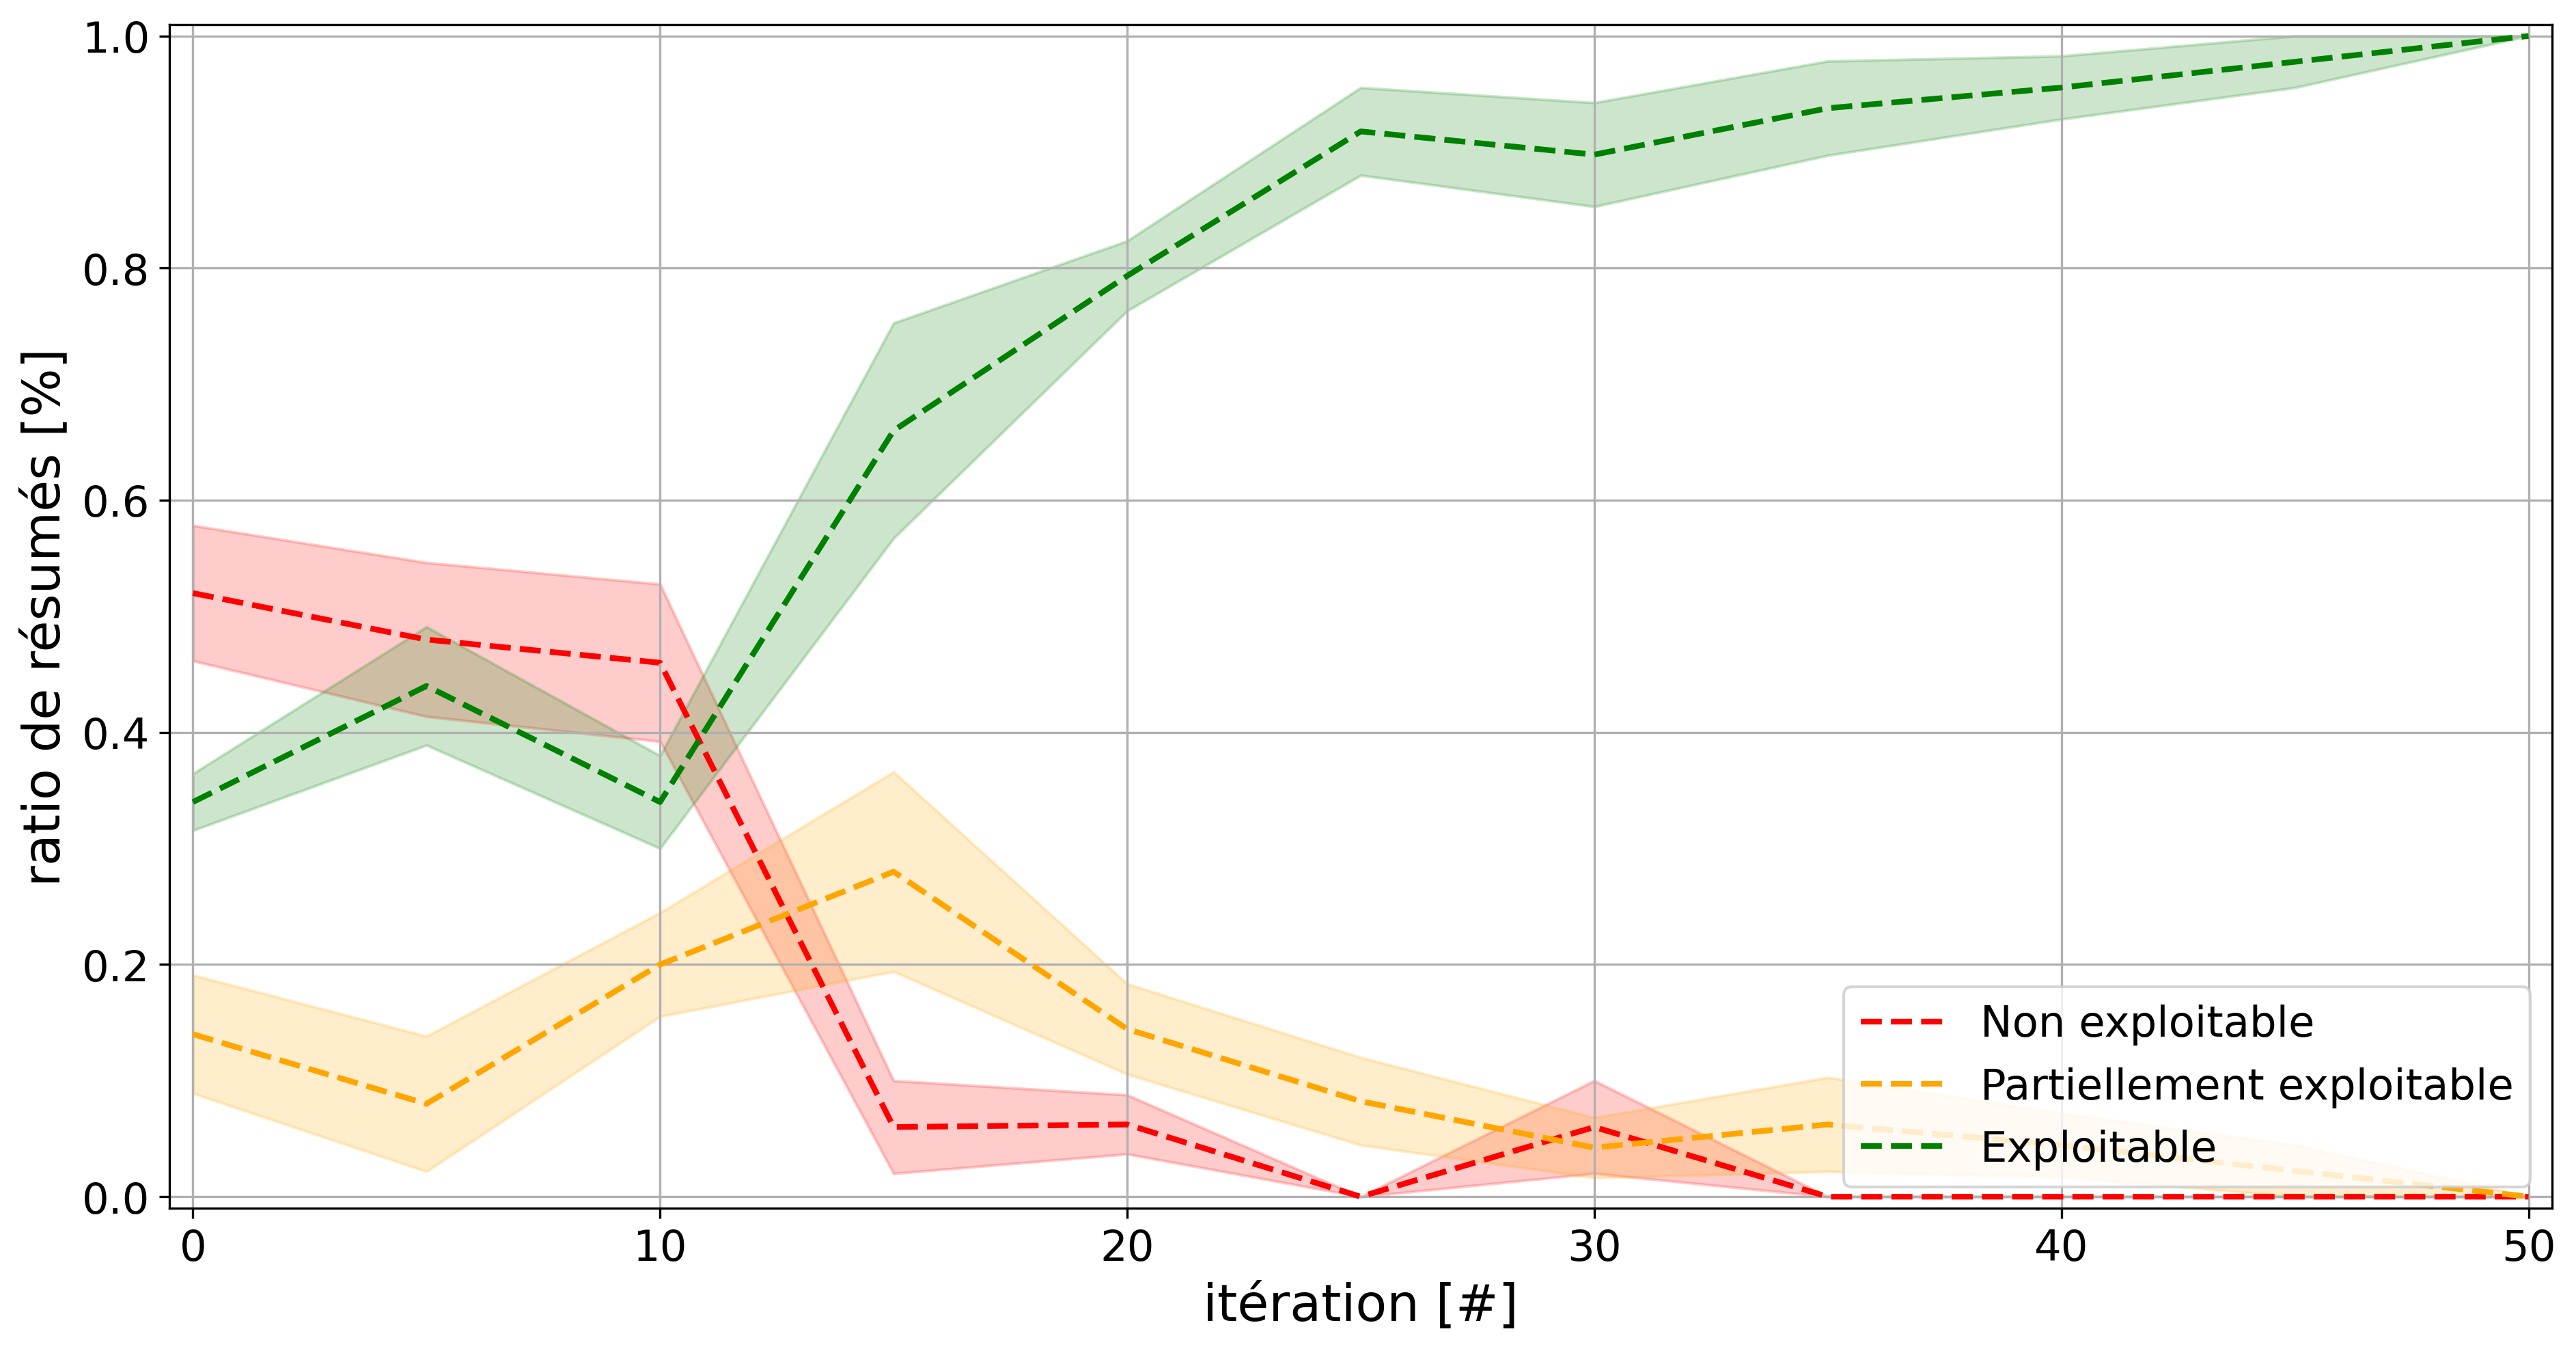
\includegraphics[width=0.95\textwidth]{figures/etude-pertinence-llm-check-resume-annotation-favori}
				\caption{Évolution de la pertinence métier moyenne en fonction du nombre d'itérations de la méthode.
				Cette pertinence, exprimée en proportion du nombre de \textit{clusters}, est estimée sur la base du résumé automatique des \textit{clusters} par un modèle de langue et est retranscrite en trois niveaux : \texttt{exploitable} en vert, \texttt{partiellement exploitable} en orange, et \texttt{non exploitable} en rouge.}
				\label{figure:4.4.3-ETUDE-PERTINENCE-RESUME-AUTOMATIQUE}
			\end{figure}
			
			% Description de deux cas d'études.
			Pour aller plus loin, reprenons les \textit{clusters} que nous avons utilisé comme cas d'étude lors de l'analyse linguistique à l'aide de la maximisation des traits (cf. sous-section~\ref{section:4.4.2-ETUDE-PERTINENCE-PATTERNS-LINGUISTIQUES}).
			
			% Exemple d'un cluster qui est bien formé dès le début.
			D'abord, reprenons l'exemple de l'évolution d'un \textit{cluster} bien formé dès l'itération $0$, précédemment détaillé dans le tableau~\ref{table:4.4.2-ETUDE-PERTINENCE-PATTERNS-LINGUISTIQUES-GESTION-SANS-CONTACT} et dont les résumés automatiques sont présentés dans le tableau~\ref{table:4.4.3-ETUDE-PERTINENCE-RESUME-AUTOMATIQUE-GESTION-SANS-CONTACT}.
			Nous constatons effectivement que les synthèses générées par le modèle identifie sans ambiguïté le thème du paiement sans contact, même si le résumé de l'itération $0$ énumère longuement les actions réalisables sur ce sujet.
			
			\todo[inline]{A REDIGER: tableau avec exemples ?}
			
			\begin{table}[!htb]
				\begin{center}
				\def\arraystretch{0.8}  % interligne
				\begin{tabular}{|c|c|}
				
				\hline
				% ENTETE DU TABLEAU
				\multicolumn{1}{|c|}{\shortstack[c]{
					Identification \\ du cluster
				}}
					& \multicolumn{1}{c|}{\shortstack[c]{
						Résumé du cluster
					}}
					\tabularnewline
					\hline
				
				% Exemple 1.1:
				{ \footnotesize Tentative: $1$ }
					& 
					\tabularnewline
				{ \footnotesize Itération: $0$ }
					& { \footnotesize La thématique traitée dans ces textes est la gestion de l'activation, }
					\tabularnewline
				{ \footnotesize Cluster: $0$ }
					& { \footnotesize la désactivation, la modification ou la nécessité d'utiliser le paiement sans contact }
					\tabularnewline
				{ \footnotesize Avis initial: }
					& { \footnotesize ou le NFC (Near Field Communication) sur les cartes de paiement bancaires. }
					\tabularnewline
				{ \footnotesize \color{colorDarkPastelGreen} \texttt{Exploitable} }
					&
					\tabularnewline
					\hline
					
				% Exemple 1.2:
				{ \footnotesize Tentative: $1$ }
					& 
					\tabularnewline
				{ \footnotesize Itération: $15$ }
					& { \footnotesize Les textes traitent de la gestion et de l'utilisation du }
					\tabularnewline
				{ \footnotesize Cluster: $0$ }
					& { \footnotesize paiement sans contact (NFC) sur les cartes bancaires. }
					\tabularnewline
				{ \footnotesize Avis initial: }
					&
					\tabularnewline
				{ \footnotesize \color{colorDarkPastelGreen} \texttt{Exploitable} }
					&
					\tabularnewline
					\hline
					
				\end{tabular}
				\end{center}
				\caption{Extrait de de l'analyse de résumés automatiques de \textit{clusters} exploitables dès la première itération.
				Ces \textit{clusters} représentent la thématique \texttt{gestion\_sans\_contact} entre l'itération $0$ (initialisation) et l'itération $15$ (atteinte de la vérité terrain).
				La seconde colonne expose le résumé obtenu en appelant un large modèle de langue (\texttt{gpt-3.5-turbo}) sur une tâche de résumé.
				}
				\label{table:4.4.3-ETUDE-PERTINENCE-RESUME-AUTOMATIQUE-GESTION-SANS-CONTACT}
			\end{table}
			
			% Exemple d'un cluster qui se forme.
			Ensuite, intéressons nous l'exemple de l'évolution des \textit{clusters} en cours de formations détaillés dans le tableau~\ref{table:4.4.2-ETUDE-PERTINENCE-PATTERNS-LINGUISTIQUES-GESTION-SANS-CONTACT} et dont les résumés automatiques sont présentés dans le tableau~\ref{table:4.4.3-ETUDE-PERTINENCE-RESUME-AUTOMATIQUE-GESTION-SANS-CONTACT}.
			À l'itération $0$, le résumé proposé est une longue énumération de $9$ thématiques différentes sur la gestion de carte bancaires : puisque le jeu de données entier traite des cartes bancaires, nous identifions clairement ce \textit{cluster} comme non exploitable.
			À l'itération $10$, nous ne distinguons plus que deux sujets principaux : le déblocage de carte, et l'utilisation de numéros de cartes virtuelles, ce qui est en accord avec notre précédente analyse.
			À partir de l'itération $15$, ces deux thématiques se retrouvent bien séparées dans deux \textit{clusters} différents, et chacune est identifiable via le résumé proposé : on note toutefois que si la thématique principale est identifiée, alors l'énumération de détails est plutôt portée sur les actions réalisables avec cette thématique ("\textit{création}", "\textit{activation}", "\textit{suppression}" pour la classe \texttt{gestion\_carte\_virtuelle}).
			
			\begin{table}[!htb]
				\begin{center}
				\def\arraystretch{0.8}  % interligne
				\begin{tabular}{|c|c|}
				
				\hline
				% ENTETE DU TABLEAU
				\multicolumn{1}{|c|}{\shortstack[c]{
					Identification \\ du cluster
				}}
					& \multicolumn{1}{c|}{\shortstack[c]{
						Résumé du cluster
					}}
					\tabularnewline
					\hline

				% Exemple 2.1:
				{ \footnotesize Tentative: $1$ }
					& 
					\tabularnewline
				{ \footnotesize Itération: $0$ }
					& { \footnotesize La thématique des textes est la gestion des cartes bancaires, incluant la sécurité, }
					\tabularnewline
				{ \footnotesize Cluster: $1$ }
					& { \footnotesize les pertes, les vols, les blocages, les récupérations, le changement ou la }
					\tabularnewline
				{ \footnotesize Avis initial: }
					& { \footnotesize commande de cartes, les garanties et assurances, les découverts, les paiements }
					\tabularnewline
				{ \footnotesize \color{colorDarkPastelRed} \texttt{Non} }
					& { \footnotesize virtuels, les numéros virtuels et les plafonds de paiement autorisés. }
					\tabularnewline
				{ \footnotesize \color{colorDarkPastelRed} \texttt{exploitable} }
					&
					\tabularnewline
					\hline
					
				% Exemple 2.2:
				{ \footnotesize Tentative: $1$ }
					& 
					\tabularnewline
				{ \footnotesize Itération: $10$ }
					& { \footnotesize Les textes traitent principalement de la gestion des cartes de paiement, }
					\tabularnewline
				{ \footnotesize Cluster: $2$ }
					& { \footnotesize de leur déblocage ou leur réactivation, et de l'utilisation de numéros }
					\tabularnewline
				{ \footnotesize Avis initial: }
					& { \footnotesize de carte virtuelle pour les achats en ligne. }
					\tabularnewline
				{ \footnotesize \color{colorCadmiumOrange} \texttt{Partiellement} }
					&
					\tabularnewline
				{ \footnotesize \color{colorCadmiumOrange} \texttt{exploitable} }
					&
					\tabularnewline
					\hline
					
				% Exemple 2.3a:
				{ \footnotesize Tentative: $1$ }
					& 
					\tabularnewline
				{ \footnotesize Itération: $15$ }
					& { \footnotesize  Les textes concernent la gestion et l'utilisation des numéros de carte virtuelle }
					\tabularnewline
				{ \footnotesize Cluster: $2$ }
					& { \footnotesize pour les achats en ligne, notamment la création, l'activation, la suppression }
					\tabularnewline
				{ \footnotesize Avis initial: }
					& { \footnotesize et la gestion de ces numéros virtuels. }
					\tabularnewline
				{ \footnotesize \color{colorDarkPastelGreen} \texttt{Exploitable} }
					&
					\tabularnewline
					\hline
					
				% Exemple 2.3b:
				{ \footnotesize Tentative: $1$ }
					& 
					\tabularnewline
				{ \footnotesize Itération: $15$ }
					& { \footnotesize La thématique traitée dans ces textes est le déblocage, le déverrouillage }
					\tabularnewline
				{ \footnotesize Cluster: $4$ }
					& { \footnotesize ou la réactivation de cartes bancaires bloquées. }
					\tabularnewline
				{ \footnotesize Avis initial: }
					&
					\tabularnewline
				{ \footnotesize \color{colorDarkPastelGreen} \texttt{Exploitable} }
					&
					\tabularnewline
					\hline
					
				\end{tabular}
				\end{center}
				\caption{Extrait de de l'analyse de résumés automatiques de \textit{clusters} évoluant de non exploitables à exploitables.
				Ces \textit{clusters} représentent la conception des thématiques \texttt{gestion\_carte\_virtuelle} et \texttt{deblocage\_carte}, entre l'itération $0$ (initialisation) et l'itération $15$ (atteinte de la vérité terrain).
				La seconde colonne expose le résumé obtenu en appelant un large modèle de langue (\texttt{gpt-3.5-turbo}) sur une tâche de résumé.
				}
				\label{table:4.4.3-ETUDE-PERTINENCE-RESUME-AUTOMATIQUE-DEBLOCAGE-CARTE-GESTION-CARTE-VIRTUELLE}
			\end{table}
			
			% Présence de quelques cas abhérants.
			De manière générale, le résumé obtenu par le modèle donne une image assez fidèle des différents \textit{clusters}.
			En effet, en considérant les $376$ \textit{clusters} évalués lors des itérations n'ayant pas encore atteint la vérité terrain, les résumés automatiques permettent d'identifient les mêmes thématiques qu'une vérification manuelle dans $85$\% des cas ($312$ \textit{clusters}).
			Concernant les $15$\% de différences, nous avons différents cas de figure :
			\begin{itemize}
				\item si le modèle génère un résumé concis, certaines thématiques peuvent être minimisées voire ignorées : par exemple, le \textit{cluster} $2$ de la tentative $3$ à l'itération $20$ contient les thématiques \texttt{consultation\_solde} et \texttt{gestion\_carte\_virtuelle}, mais seule la seconde est mentionnée dans le résumé ;
				\item à l'inverse, les données aberrantes ou isolées d'un \textit{cluster} peuvent influencer le résumé, donnant l'illusion que plusieurs thématiques sont présentes alors qu'une seule ne l'est réellement (voir le \textit{cluster} $9$ de la tentative $5$ à l'itération $15$, où les thématiques \texttt{couverture\_assurrance} et \texttt{deblocage\_carte} représentent $4$ questions sur $51$ et sont néanmoins citées dans le résumé) ;
				\item le résumé issu du large modèle de langue peut aussi identifier des thématiques auquel l'expert n'aurait pas pensé : c'est le cas dans les \textit{clusters} $7$ et $8$ de la tentative $1$ à l'itération $0$, où les thématiques \texttt{gestion\_carte\_mastercard} et \texttt{gestion\_carte\_visa} sont proposées dans la synthèse, mais n'aurait pas été par un expert (il n'y a pas de différences aussi significatives entre les deux réseaux de cartes bancaires pour justifier une gestion séparée) ;
				\item enfin, le modèle peut aussi générer des hallucinations n'ayant rien à voir avec les données en entrée : c'est le cas avec le cluster $9$ de la tentative $2$ à l'itération $10$, où le cluster est composé de $2$ questions (« \textit{Comment obtenir une Mastercard ?} » et « \textit{Désactiver les numéros virtuels.} ») et où le résumé parle de "\textit{sécurisation des transactions bancaires}"
			\end{itemize}

		%%% Discussion
		\subsubsection{Discussion}
			
			% Rappel de l'objectif.
			Dans cette dernière étude sur l'évaluation de la valeur métier d'un résultat de \textit{clustering}, nous avons adapté les capacités d'un large modèle de langue pour résumer les thématiques présentes dans chaque regroupement de questions.
			Comme lors de la vérification manuelle (cf. sous-section~\ref{section:4.4.1-ETUDE-PERTINENCE-VERIFICATION-MANUELLE}), ces résumés ont été annotés en trois catégories : exploitable, partiellement exploitable et non exploitable.
		
			% Remaques expérience utilisateur.
			La principale remarque concerne la facilité d'utilisation et le gain de temps d'analyse qui est possible avec une telle approche.
			En effet, en disposant d'une synthèse écrite qui tiens en une ou deux phrases, nous avons là un moyen de réduire grandement la pénibilité du travail d'analyse réalisé par les experts métiers.
			Bien que ces résumés peuvent avoir quelques biais (hallucinations, oublis, erreurs de reformulations), ils permettent de donner rapidement un aperçu du contenu des \textit{clusters} obtenus.
			De plus, la structure du résumé peut parfois aiguiller l'analyse de la qualité du regroupement des questions, notamment car le modèle met généralement l'emphase sur les thématiques principales et énumère les thématiques secondaires à la fin de sa génération.
			
			% Conclusions et suggestion.
			\todo[inline]{A REDIGER: rappeler quelques soucis de la générations}